% !TeX spellcheck = cs_CZ
  
Nyní si demonstrujeme užití pohybových rovnic při popisu trajektorie, libovolného bodu na 
železničním kole, které se odvaluje po kolejnici \textbf{bez} smyku. Na obrázku \ref{fyz:fig0142} 
vidíme, že železniční kola jsou opatřena \emph{okolky}, která slouží jako bezpečnostní prvek proti 
vykolejení a pro hladký průjezd kolejových spojek, výhybek apod. Úlohu můžeme formulovat pro různé 
body, které mají vzdálenost od středu kola menší, větší, nebo rovnou poloměru nákolku. Otázka zní, 
jak bude jejich trajektorie rozvinutá v čase vypadat.

\begin{figure}[ht!]  %\ref{fyz:fig0142}
  \centering
  \luafigure[0.6]{fyz_fig0142.jpg}
  \caption{Typické železniční dvojkolí se skládá ze dvou kol nalisovaný na nápravu. Na obrázku je
          nákres kola a části kolejnice: \(1\ldots\) okolek, \(2\ldots\) nákolek, \(3\ldots\) plocha
          odvalování, kredit: \wikiOkolek. K příkladu \ref{fyz:fey_exam003}.}
  \label{fyz:fig0142}
\end{figure}

\begin{mdframed}[style=mdexam]
  \begin{example}\label{fyz:fey_exam003}
    Kolo vagónu se valí po vodorovné kolejnici. Uvažujme bod, který je v počátečním okamžiku pod
    středem kola ve vzdálenosti, která může být menší, rovna nebo větší než vzdálenost středu kola
    od kolejnice.

    {\centering
      \captionsetup{type=figure}
      \luafigure[0.7]{fyz_fig0141.pdf}
      \captionof{figure}{Kolo vagónu a tři možné polohy bodu}
      \label{fyz:fig0141}
    \par}
    \vspace{0.5em}
    Určeme parametrické rovnice dráhy zvoleného bodu, složky rychlosti a její velikost, složky 
    zrychlení a jeho velikost, tečné a normálové zrychlení a poloměr křivosti dráhy. 
    \cite[p.~11]{Slavik}
    \vspace{1em}
    \newline
    \textbf{Řešení}: Obvodová rychlost v místě dotyku s kolejnicí je \(v=\omega R\), což vzhledem k
    předpokladu o valení představuje posuvnou rychlost kola. Parametrické rovnice pro střed kola
    jsou pak
    \begin{subequations}\label{mech:eq_wheel_center}
      \begin{align}
        x_s &= \omega R t \\
        y_s &= R
      \end{align}
    \end{subequations}

    {\centering
      \captionsetup{type=figure}
      \luafigure[1]{fyz_fig0143.pdf}
      \captionof{figure}{Náčrt pro odvození parametrických rovnic pohybu libovolně zvoleného bodu na 
                kole vagónu}
      \label{fyz:fig0143}
    \par}
    \vspace{0.5em}
    Uvažovaný bod \(B_3\) na obr. \ref{fyz:fig0143} je ve své nové pozici v čase \(t_1\) posunut vůči
    středu o vzdálenost \(r\cdot\sin\omega t\) ve směru osy \(x\) a o vzdálenost \(r\cdot\cos\omega
    t\) ve směru osy \(y\). Z obrázku \ref{fyz:fig0143} lze odvodit následující rovnice pro
    souřadnice libovolného bodu \(B\) na kole vagónu.  
            
      \begin{itemize}
        \item ve směru osy \(x\):
        \begin{align*}
          x &= x_s + x'                        \\
          x &= x_s + r\cos(\psi-\frac{\pi}{2}) \\
          x &= x_s + r\sin\psi                 \\
          x &= \omega R t + r\sin\omega t
        \end{align*}
        \end{itemize}  


    \begin{itemize}
        \item ve směru osy \(y\): 
        \begin{align*}
          y &= y_s - y'                        \\
          y &= y_s - r\sin(\psi-\frac{\pi}{2}) \\
          y &= y_s + r\cos\psi                 \\
          y &= R + r\cos\omega t
        \end{align*}
      \end{itemize}

    takže, parametrické rovnice dráhy mají tvar \textbf{cykloidy}:
    \begin{equation*}
      x = \omega R t + r\sin\omega t  \qquad y = R + r\cos\omega t
    \end{equation*}
    \begin{itemize}
      \item Složky rychlosti:
        \begin{gather*}
          \begin{align*} 
          v_x &= \frac{dx}{dt} = \omega R + r\omega\cos\omega t                       \\
          v_y &= \frac{dy}{dt} = -r\omega\sin\omega t                                 \\
          v   &= \sqrt{v_x^2 + v_y^2}= \omega\sqrt{R^2 + 2Rr\cos\omega t + r^2}
          \end{align*}
        \end{gather*}
      \item Složky zrychlení:
        \begin{gather*}
          \begin{align*}
            a_x &= \frac{dv_x}{dt} = -r\omega^2\sin\omega t                           \\
            a_y &= \frac{dv_y}{dt} = -r\omega^2\cos\omega t                           \\
            a   &= \sqrt{a_x^2 + a_y^2}= r\omega^2\sqrt{\sin^2\omega t + 
                  \cos^2\omega t} = r\omega^2
          \end{align*}
        \end{gather*}
        Tento výsledek je superpozicí rovnoměrného kruhového a rovnoměrného přímočarého pohybu.
      \item \textbf{Tečné zrychlení} \(a_t\) dostaneme derivací velikosti rychlosti
        \begin{equation*}
          a_t = \frac{dv}{dt} = -\cdot\frac{2Rr\omega^2\sin\omega t }{2\sqrt{R^2 + 
                  2Rr\cos\omega t + r^2}}
        \end{equation*}
      \item \textbf{Normálové zrychlení} \(a_n\) získáme užitím Pythagorovy věty
        \begin{align*}
          a_n &= \sqrt{a^2 - a_t^2}                                                 \\
          a_n &= \sqrt{(r\omega^2)^2-\left(
                \frac{Rr\omega^2\sin\omega t}
                      {\sqrt{R^2 + 2Rr\cos\omega t + r^2}}\right)^2}
        \end{align*}
      \item \textbf{Poloměr křivosti} $R_0$ dostaneme ze vztahu $a_n=\frac{v^2}{R_0}$:
        \begin{equation*}
            R_0 =  \dfrac{\omega^2\cdot(R^2 + 2Rr\cos\omega t + r^2)}{\sqrt{r^2\omega^4 - 
                    \dfrac{R^2r^2\omega^4\sin^2\omega t}{R^2 + 2Rr\cos\omega t + r^2}}}
        \end{equation*}
        Poloměr křivosti není roven vzdálenosti od středu kola r: drahou bodu není kružnice, nýbrž 
        cykloida (viz obr. \ref{fyz:fig0140}). Pokud bod pevně spojený s kružnicí leží na 
        jejím obvodu, pak při valení této kružnice po přímce opisuje tento bod \textbf{prostou} 
        (obecnou) cykloidu. 
    \end{itemize}
    
    \begin{gather*}
      \begin{align*}
        (x - \omega R t)^2            &= r^2\sin^2\omega t                          \\
        (y-R)^2                       &= r^2\cos\omega t                            \\
        (x - \omega R t)^2 + (y-R)^2  &= r^2\sin^2\omega t + r^2\cos\omega t        \\
        (x - \omega R t)^2 + (y-R)^2  &= r^2 \quad                                  \\
        \shortintertext{kde \(t = \frac{1}{\omega}\arccos\frac{y-R}{r}\)}
        \Aboxed{\left(x - R\arccos\frac{y-R}{r}\right)^2 + (y-R)^2  &= r^2}
      \end{align*}
    \end{gather*}

    {\centering
      \captionsetup{type=figure}
      \luafigure[1]{fyz_fig0140.pdf}
  %   % file: fyz_fig0140.tex
% This file was created by matlab2tikz.
%
%The latest updates can be retrieved from
%http://www.mathworks.com/matlabcentral/fileexchange/22022-matlab2tikz-matlab2tikz
%where you can also make suggestions and rate matlab2tikz.

\documentclass[11pt]{standalone}
\usepackage{xltxtra}
\usepackage{siunitx}
\usepackage[usenames,x11names]{xcolor}
\usepackage{tikz}
\usepackage{pgfplots}
  \pgfplotsset{compat=newest}
\usepackage{amsmath}

\begin{document}

    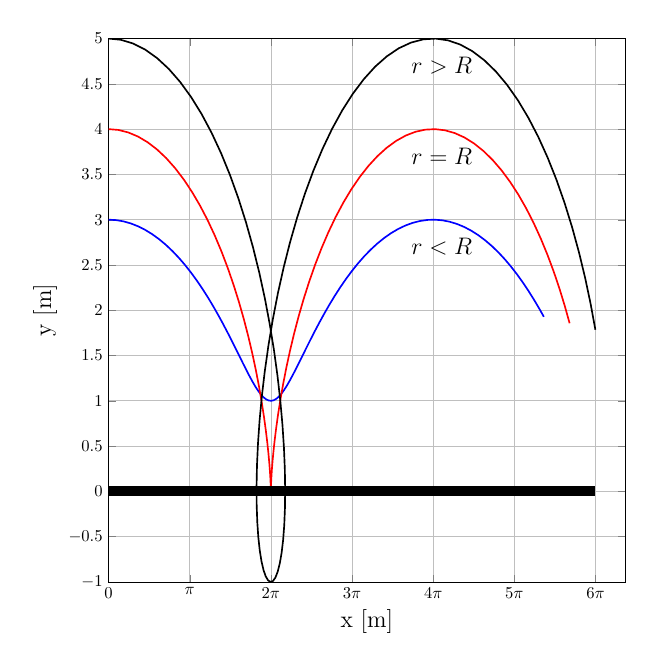
\begin{tikzpicture}[scale=0.6]
    
    \begin{axis}[%
      width=4.306in,
      height=4.528in,
      at={(0.722in,0.611in)},
      scale only axis,
      xmin=0,
      xmax=20,
      xtick={0,3.14159265358979,6.28318530717959,9.42477796076938,12.5663706143592,15.707963267949,18.8495559215388,21.9911485751286,25.1327412287183},
      xticklabels={{0},{\(\pi\)},{\(2\pi\)},{\(3\pi\)},{\(4\pi\)},{\(5\pi\)},{\(6\pi\)},{\(6\pi\)},{\(8\pi\)}},
      xlabel={\Large x [m]},
      xmajorgrids,
      ymin=-1,
      ymax=5,
      ylabel={\Large y [m]},
      ymajorgrids,
      axis background/.style={fill=white}
    ]
    \addplot [color=blue,solid,line width=1.0pt,forget plot]
      table[row sep=crcr]{%
    0  3\\
    0.286333831818311  2.99544401045211\\
    0.571798855564011  2.98181755588998\\
    0.855534179725487  2.95924480028271\\
    1.13669467377758  2.92793142610753\\
    1.41445866899325  2.88816276017536\\
    1.68803544547188  2.84030117373882\\
    1.95667243716243  2.78478278057302\\
    2.2196620892296  2.72211346311592\\
    2.47634830527867  2.65286426287812\\
    2.72613242569217  2.57766617712461\\
    2.96847868260375  2.4972044092408\\
    3.20291908180385  2.41221212517367\\
    3.42905766709306  2.32346377283893\\
    3.64657412822683  2.23176802536784\\
    3.85522671957563  2.13796041249453\\
    4.05485446290616  2.04289570722652\\
    4.24537861421158  1.94744013717097\\
    4.42680338122528  1.85246349148679\\
    4.59921588508011  1.75883119538405\\
    4.76278536646244  1.66739642438753\\
    4.91776164349451  1.57899233021916\\
    5.06447283539702  1.49442444913699\\
    5.20332237267356  1.41446336190563\\
    5.33478532106034  1.33983767228038\\
    5.45940405273711  1.27122736798514\\
    5.57778330424324  1.20925762467838\\
    5.69058466613095  1.1544931093657\\
    5.79852055456608  1.10743283516581\\
    5.90234771980685  1.06850561431346\\
    6.00286035071135  1.03806615083132\\
    6.10088283810525  1.01639180847432\\
    6.19726226294983  1.00368008339693\\
    6.29286067775796  1.00004680457233\\
    6.38854725158968  1.00552507836121\\
    6.48519035020179  1.02006498684734\\
    6.58364962351733  1.04353404268853\\
    6.6847681725134  1.07571839633857\\
    6.78936486690267  1.11632478463977\\
    6.89822688360971  1.16498320303079\\
    7.01210253403131  1.22125027702041\\
    7.13169444543863  1.28461330220665\\
    7.25765315865222  1.35449491602859\\
    7.3905712003277  1.43025835868189\\
    7.5309776838652  1.51121327526087\\
    7.67933348813913  1.59662200625796\\
    7.83602705797955  1.68570630910172\\
    8.00137086467097  1.77765444948689\\
    8.17559855872052  1.87162859788037\\
    8.35886284083946  1.96677246380645\\
    8.55123407053743  2.06221909834774\\
    8.75269962500815  2.15709879376552\\
    8.96316401414808  2.25054700825854\\
    9.1824497506603  2.3417122436498\\
    9.41029896731505  2.42976380422016\\
    9.64637576663052  2.51389936599034\\
    9.89026928156366  2.59335228748028\\
    10.1414974193222  2.66739859533028\\
    10.3995112541838  2.73536358113108\\
    10.6637000292963  2.79662794935282\\
    10.9333967218807  2.85063346035295\\
    11.2078841211294  2.89688801704418\\
    11.4864013634157  2.93497014887285\\
    11.7681508652674  2.96453285224982\\
    12.0523055909307  2.98530675243991\\
    12.3380165883028  2.99710255809884\\
    12.6244207245654  2.99981278609203\\
    12.9106485510334  2.99341274087867\\
    13.1958322255526  2.97796073953694\\
    13.4791134202598  2.95359758038007\\
    13.7596511426479  2.920545260005\\
    14.0366293986721  2.87910495046405\\
    14.3092646280711  2.82965425499148\\
    14.576812844151  2.7726437672907\\
    14.8385764129771  2.7085929657339\\
    15.0939104101996  2.63808547988592\\
    15.3422284975907  2.5617637724839\\
    15.5830082657464  2.48032328533025\\
    15.8157959942697  2.39450610244145\\
    16.0402107860621  2.30509418819405\\
    16.2559480380492  2.21290226208159\\
    16.4627822167181  2.1187703750076\\
    16.6605689131738  2.02355625475934\\
    16.8492461589901  1.92812749041013\\
    };
    \node[right, align=left, text=black]
    at (axis cs:11.5,2.7) {\Large \(r<R\)};
    \addplot [color=red,solid,line width=1.0pt,forget plot]
      table[row sep=crcr]{%
    0  4\\
    0.381681731926347  3.99088802090423\\
    0.761625847707474  3.96363511177995\\
    1.13811056432015  3.91848960056541\\
    1.50944562071406  3.85586285221506\\
    1.87398767943513  3.77632552035071\\
    2.23015530068212  3.68060234747763\\
    2.57644335235294  3.56956556114604\\
    2.911436724777  3.44422692623183\\
    3.23382322516487  3.30572852575625\\
    3.54240553428159  3.15533235424922\\
    3.83611211639449  2.99440881848161\\
    4.1140069830844  2.82442425034734\\
    4.37529822195256  2.64692754567785\\
    4.61934521250981  2.46353605073567\\
    4.84566446349715  2.27592082498905\\
    5.05393401844793  2.08579141445304\\
    5.24399638934849  1.89488027434194\\
    5.41585999166562  1.70492698297359\\
    5.56969906766501  1.51766239076811\\
    5.70585209871938  1.33479284877505\\
    5.82481872107327  1.15798466043832\\
    5.92725517316801  0.988848898273986\\
    6.01396831601081  0.828926723811252\\
    6.08590828107409  0.679675344560767\\
    6.14415981271736  0.542454735970277\\
    6.18993238401934  0.418515249356769\\
    6.22454917608448  0.308986218731405\\
    6.24943502124447  0.214865670331623\\
    6.26610342001574  0.137011228626926\\
    6.27614275011447  0.0761323016626385\\
    6.28120179319199  0.0327836169486335\\
    6.28297471117087  0.00736016679385365\\
    6.28318560907687  9.36091446517295e-05\\
    6.28357282503002  0.0110501567224259\\
    6.28587309054397  0.0401299736946852\\
    6.29180570546478  0.0870680853770696\\
    6.30305687174664  0.151436792677134\\
    6.32126432881491  0.232649569279539\\
    6.34800243051873  0.329966406061573\\
    6.38476779965164  0.442500554040812\\
    6.432965690756  0.569226604413309\\
    6.49389718547292  0.708989832057179\\
    6.56874733711361  0.860516717363772\\
    6.65857437247832  1.02242655052173\\
    6.76430004931591  1.19324401251592\\
    6.88670125728648  1.37141261820345\\
    7.02640293895904  1.55530889897378\\
    7.18387239534787  1.74325719576073\\
    7.35941502787546  1.9335449276129\\
    7.55317155556114  2.12443819669547\\
    7.7651167327923  2.31419758753104\\
    7.99505957936188  2.50109401651708\\
    8.24264512067606  2.6834244872996\\
    8.50735762227529  2.85952760844031\\
    8.78852528919594  3.02779873198067\\
    9.08532638735196  3.18670457496056\\
    9.39679673115867  3.33479719066056\\
    9.72183846917169  3.47072716226216\\
    10.0592300876863  3.59325589870564\\
    10.4076375411449  3.7012669207059\\
    10.765626407932  3.79377603408835\\
    11.1316749607943  3.8699402977457\\
    11.5041880327875  3.92906570449965\\
    11.8815115524038  3.97061350487982\\
    12.2619476154377  3.99420511619768\\
    12.6437699562527  3.99962557218406\\
    13.0252396774784  3.98682548175734\\
    13.4046210948066  3.95592147907389\\
    13.7801975525107  3.90719516076014\\
    14.1502870655765  3.84109052001\\
    14.5132576459148  3.75820990092809\\
    14.8675421730024  3.65930850998295\\
    15.2116526734519  3.54528753458141\\
    15.5441938793939  3.4171859314678\\
    15.8638759421286  3.27617095977184\\
    16.1695261852006  3.1235275449678\\
    16.4600997898016  2.96064657066049\\
    16.7346893151381  2.7890122048829\\
    16.9925329670126  2.6101883763881\\
    17.2330215392765  2.42580452416318\\
    17.455703964904  2.23754075001519\\
    17.6602914261051  2.04711250951867\\
    17.8466599860274  1.85625498082027\\
    };
    \node[right, align=left, text=black]
    at (axis cs:11.5,3.7) {\Large \(r=R\)};
    \addplot [color=black,solid,line width=1.0pt,forget plot]
      table[row sep=crcr]{%
    0  5\\
    0.477029632034383  4.98633203135634\\
    0.951452839850936  4.94545266766993\\
    1.42068694891481  4.87773440084812\\
    1.88219656765054  4.7837942783226\\
    2.33351668987702  4.66448828052607\\
    2.77227515589235  4.52090352121645\\
    3.19621426754345  4.35434834171905\\
    3.6032113603244  4.16634038934775\\
    3.99129814505107  3.95859278863437\\
    4.35867864287101  3.73299853137383\\
    4.70374555018523  3.49161322772241\\
    5.02509488436496  3.236636375521\\
    5.32153877681206  2.97039131851678\\
    5.5921162967928  2.69530407610351\\
    5.83610220741866  2.41388123748358\\
    6.05301357398969  2.12868712167956\\
    6.2426141644854  1.84232041151291\\
    6.40491660210596  1.55739047446038\\
    6.54018225024991  1.27649358615216\\
    6.64891883097633  1.00218927316258\\
    6.73187579865202  0.736976990657473\\
    6.79003751093899  0.48327334741098\\
    6.82461425934806  0.243390085716878\\
    6.83703124108784  0.0195130168411501\\
    6.82891557269761  -0.186317896044585\\
    6.80208146379544  -0.372227125964847\\
    6.75851368603802  -0.536520671902893\\
    6.70034948792286  -0.677701494502565\\
    6.62985912022463  -0.794483157059612\\
    6.54942514951759  -0.885801547506042\\
    6.46152074827874  -0.95082457457705\\
    6.36868715939191  -0.98895974980922\\
    6.27351054039578  -0.999859586283022\\
    6.17859839847037  -0.983424764916361\\
    6.08655583088616  -0.939805039457972\\
    5.99996178741223  -0.869397871934396\\
    5.92134557097988  -0.772844810984298\\
    5.85316379072715  -0.651025646080691\\
    5.79777797742774  -0.50505039090764\\
    5.75743306527198  -0.336249168938781\\
    5.73423693607337  -0.146160093380037\\
    5.73014121229362  0.0634847480857685\\
    5.74692347389951  0.290775076045659\\
    5.78617106109144  0.533639825782596\\
    5.84926661049269  0.789866018773876\\
    5.93737545659341  1.05711892730517\\
    6.05143501324711  1.33296334846066\\
    6.19214623197522  1.6148857936411\\
    6.35996721491147  1.90031739141935\\
    6.55510904058485  2.18665729504321\\
    6.77753384057645  2.47129638129656\\
    7.02695514457569  2.75164102477562\\
    7.30284049069182  3.02513673094941\\
    7.60441627723552  3.28929141266047\\
    7.93067481176137  3.54169809797101\\
    8.28038349314025  3.78005686244085\\
    8.65209604299518  4.00219578599084\\
    9.04416568415957  4.20609074339324\\
    9.45476014607637  4.38988384805846\\
    9.8818783604091  4.55190038105885\\
    10.3233686947346  4.69066405113253\\
    10.776948558173  4.80491044661855\\
    11.2402252003075  4.89359855674947\\
    11.7107175138769  4.95592025731973\\
    12.1858786425726  4.99130767429652\\
    12.6631191879399  4.9994383582761\\
    13.1398308039234  4.980238222636\\
    13.6134099640606  4.93388221861083\\
    14.0812816847616  4.86079274114022\\
    14.5409229885052  4.76163578001499\\
    14.9898858931575  4.63731485139214\\
    15.4258197179337  4.48896276497443\\
    15.8464925027528  4.31793130187211\\
    16.2498113458106  4.1257788972017\\
    16.6338414740577  3.91425643965775\\
    16.9968238728105  3.6852913174517\\
    17.3371913138569  3.44096985599074\\
    17.6535826360064  3.18351830732435\\
    17.944855147963  2.91528256458215\\
    18.2100950405038  2.63870678624476\\
    18.4486257130899  2.35631112502279\\
    18.6600139390365  2.07066876427801\\
    18.8440738130648  1.7843824712304\\
    };
    \node[right, align=left, text=black]
    at (axis cs:11.5,4.7) {\Large\(r>R\)};
    \addplot [color=black,solid,line width=6.0pt,forget plot]
      table[row sep=crcr]{%
    0  0\\
    0.477029632034383  0\\
    0.951452839850936  0\\
    1.42068694891481  0\\
    1.88219656765054  0\\
    2.33351668987702  0\\
    2.77227515589235  0\\
    3.19621426754345  0\\
    3.6032113603244  0\\
    3.99129814505107  0\\
    4.35867864287101  0\\
    4.70374555018523  0\\
    5.02509488436496  0\\
    5.32153877681206  0\\
    5.5921162967928  0\\
    5.83610220741866  0\\
    6.05301357398969  0\\
    6.2426141644854  0\\
    6.40491660210596  0\\
    6.54018225024991  0\\
    6.64891883097633  0\\
    6.73187579865202  0\\
    6.79003751093899  0\\
    6.82461425934806  0\\
    6.83703124108784  0\\
    6.82891557269761  0\\
    6.80208146379544  0\\
    6.75851368603802  0\\
    6.70034948792286  0\\
    6.62985912022463  0\\
    6.54942514951759  0\\
    6.46152074827874  0\\
    6.36868715939191  0\\
    6.27351054039578  0\\
    6.17859839847037  0\\
    6.08655583088616  0\\
    5.99996178741223  0\\
    5.92134557097988  0\\
    5.85316379072715  0\\
    5.79777797742774  0\\
    5.75743306527198  0\\
    5.73423693607337  0\\
    5.73014121229362  0\\
    5.74692347389951  0\\
    5.78617106109144  0\\
    5.84926661049269  0\\
    5.93737545659341  0\\
    6.05143501324711  0\\
    6.19214623197522  0\\
    6.35996721491147  0\\
    6.55510904058485  0\\
    6.77753384057645  0\\
    7.02695514457569  0\\
    7.30284049069182  0\\
    7.60441627723552  0\\
    7.93067481176137  0\\
    8.28038349314025  0\\
    8.65209604299518  0\\
    9.04416568415957  0\\
    9.45476014607637  0\\
    9.8818783604091  0\\
    10.3233686947346  0\\
    10.776948558173  0\\
    11.2402252003075  0\\
    11.7107175138769  0\\
    12.1858786425726  0\\
    12.6631191879399  0\\
    13.1398308039234  0\\
    13.6134099640606  0\\
    14.0812816847616  0\\
    14.5409229885052  0\\
    14.9898858931575  0\\
    15.4258197179337  0\\
    15.8464925027528  0\\
    16.2498113458106  0\\
    16.6338414740577  0\\
    16.9968238728105  0\\
    17.3371913138569  0\\
    17.6535826360064  0\\
    17.944855147963  0\\
    18.2100950405038  0\\
    18.4486257130899  0\\
    18.6600139390365  0\\
    18.8440738130648  0\\
    };
    
    \addplot [color=black,solid,line width=6.0pt,forget plot]
      table[row sep=crcr]{%
    0  0\\
    18.8440738130648  0\\
    };
    \end{axis}
  \end{tikzpicture}%
\end{document}
      \captionof{figure}{Cykloida: pro $B_2\ldots r=R$ je cykloida prostá; $B_3\ldots r>R$
                cykloida prodloužená; $B_1\ldots r<R$ cykloida zkrácená; \texttt{[cykloida.m]} }
      \label{fyz:fig0140}
      \par}       
      \vspace{1em}
    
    Z obrázku \ref{fyz:fig0140} je také patrné, že pokud bod pevně spojený s kutálející se kružnicí 
    neleží na obvodu této kružnice, ale jeho vzdálenost od středu kružnice o poloměru \(R\)  je 
    \(r\) , pak pro \(r<R\) získáme \textbf{cykloidu zkrácenou} a pro \(r>R\)  \textbf{cykloidu 
    prodlouženou}.
      
    %---------------------------------------------------------------
    \lstinputlisting[%
      style=luaMatlabStyle, 
      caption={Výpočet křivky cykloidy pro pro tři různé body.}
    ]{../src/FYZ/matlab/cicloid.m}
    %---------------------------------------------------------------

    %---------------------------------------------------------------
    % \tikzexternaldisable
    %   % !TeX spellcheck = cs_CZ

% note:
% ~~~~~~
% This figure uses expl3 package for coordinate calculating !!!
%\usepackage{expl3}                     % fpeval
%\ExplSyntaxOn
%\cs_set_eq:NN \fpeval \fp_eval:n
%\ExplSyntaxOff
%-------------------------------------------------------------------------------------------------
\def\xmin{0}
\def\xmax{8.5}
\def\ymin{-0.75}
\def\ymax{+2}
\def\zero{0}
\def\R{0.5}
\def\r{0.5}
\def\omega{4/3.14}
\def\angle{360}

{\centering
 \captionsetup{type=figure}
\begin{animateinline}
 [autoplay,
  palindrome,
  begin={
    \begin{tikzpicture}
      \useasboundingbox (\xmin,\ymin) rectangle (\xmax,\ymax);

      \draw [step=1cm, black!40!white, very thin] (\xmin cm,\ymin cm) grid (\xmax cm,\ymax cm);
      \draw [red, thick,  domain=0:6*pi, samples=100] 
        plot ({\omega*\R*\x + \r*sin(deg(\omega*\x))}, {\R+\r*cos(deg(\omega*\x))} );
        
      \draw [Mahogany, thick,  domain=0:6*pi, samples=100] 
        plot ({\omega*\R*\x + 1.5*\r*sin(deg(\omega*\x))}, {\R+1.5*\r*cos(deg(\omega*\x))} );
        
      \draw [orange, thick,  domain=0:6*pi, samples=100] 
        plot ({\omega*\R*\x + 0.4*\r*sin(deg(\omega*\x))}, {\R+0.4*\r*cos(deg(\omega*\x))} );
        
      \draw[black, thick] (\xmin cm,\ymin cm) rectangle (\xmax cm,\ymax cm);
    
      \draw [Sepia,line width=0.5mm] (\xmin,0) -- (\xmax,0);
        \foreach \x/\xtext in {1/1,2/2,3/3,4/4,5/5,6/6,7/7,8/8}
          \draw (\x cm,-3pt) -- (\x cm,2pt) node[below, yshift=-1mm, fill=white] {\xtext};
        },
  end={\end{tikzpicture}}
]{5}
  \multiframe{40}{nstep=0.1+20}{% 
    % wheel
    \filldraw[fill=black!40!white, draw=black, opacity=0.2] 
      (\nstep/57.295/3.14*2, \R cm) circle (\R cm);
    %point 1
    \filldraw[fill=red!40!white, draw=black] (\fpeval{\omega*\R*\nstep/57.295 + 
       1.0*\r*sin(deg(\omega*\nstep))},\fpeval{\R+1.0*\r*cos(deg(\omega*\nstep))}) circle (0.5 mm);
    %point 2
    \filldraw[fill=red!40!white, draw=black] (\fpeval{\omega*\R*\nstep/57.295 + 
       1.5*\r*sin(deg(\omega*\nstep))},\fpeval{\R+1.5*\r*cos(deg(\omega*\nstep))}) circle (0.5 mm);
    %point 3
    \filldraw[fill=red!40!white, draw=black] (\fpeval{\omega*\R*\nstep/57.295 + 
       0.4*\r*sin(deg(\omega*\nstep))},\fpeval{\R+0.4*\r*cos(deg(\omega*\nstep))}) circle (0.5 mm);
}
\end{animateinline}
\captionof{figure}{Animace parametrických rovnic pohybu libovolně zvoleného bodu na kole}
\label{fyz:fig0144}
\par}
    % \tikzexternalenable
    %---------------------------------------------------------------      
  \end{example}
\end{mdframed}